\section{Arbejdsfordeling}
Projektet blev opdelt i to blokke: server og applikation. Da der blev valgt Xamarin som platform til applikationen og Firebase til serveren, skulle gruppen arbejde med nye tekonologier. Dette gav gruppens medlemmer en god udvikling i projektet, med en stejl læringskurve.

Ao arbejdede med serveropsætningen, da han tidligere havde deltaget i nogle meet ups omkring Firebase og derfor havde en interesse for dette. Begge gruppemedlemmer fulgte en smartphone kursus på 6. semester, som der kunne drages nytte af under udviklingen af applikationen. Der var også nyt stof, da det var en iOS applikation, som skulle udvikles, hvor kurset på 6. semester var i Android udvikling. 

For at holde overblikket over arbejdsopgaverne, blev der brugt et kanban board. Dette værktøj havde til formål at give et indblik i, hvad hvert enkelt gruppemedlem arbejdede med i øjeblikket. Kanban boardet var det centrale punkt i daglig stand up møder hver morgen, hvor man gennemgik, hvad hvert medlem havde arbejdt med i går og hvad man skulle arbejdes videre med i dag. \\
På figur \ref{fig:Kanbanboard} ses et billede af det overordnede fysiske kanban board. For mere detaljeret kanban board, gå til bilag og se kanban screenshots. \\

\begin{figure} [H]
	\begin{center}
		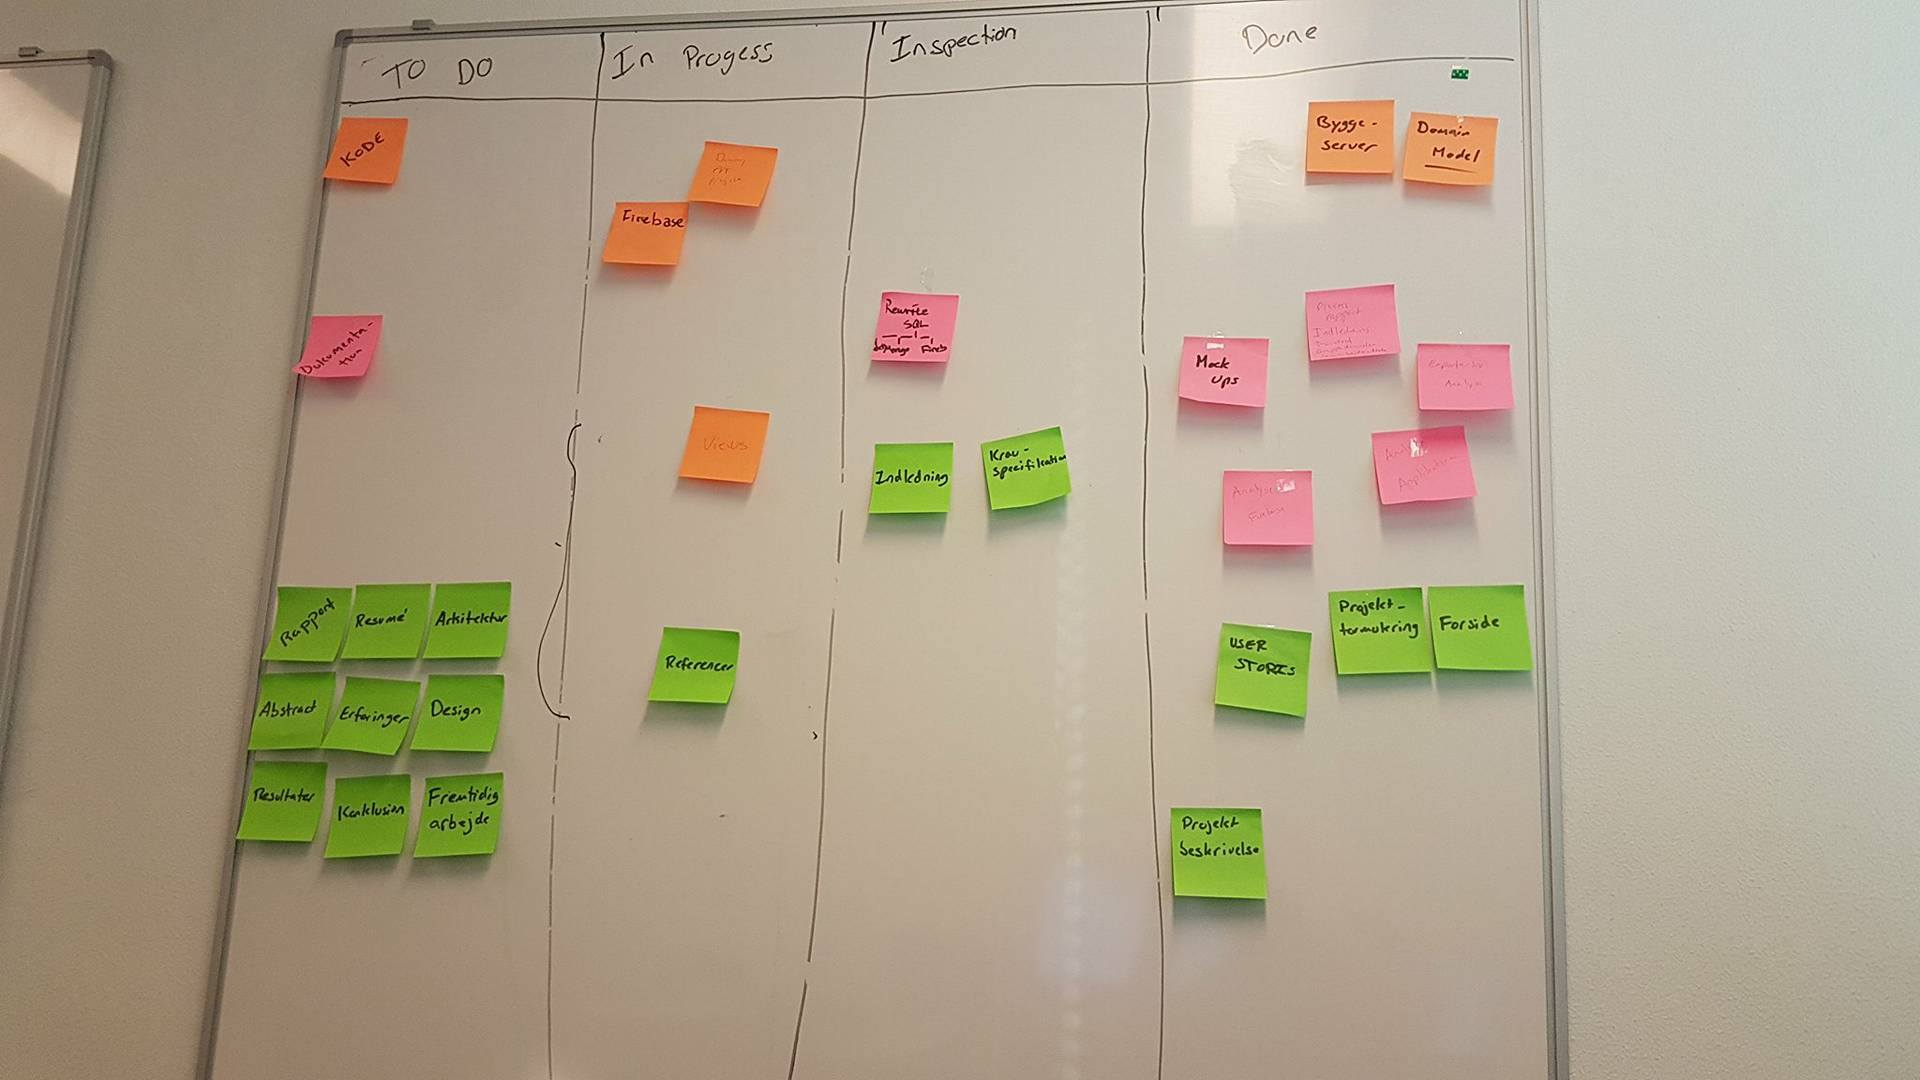
\includegraphics[height=8cm, width=12cm]{Arbejdsfordeling/ScrumBoard}
	\end{center}
	\caption{Kanban board}
	\label{fig:Kanbanboard}
\end{figure}

For en yderlige beskrivelse af hvem der har lavet hvad, henvises til 'Hvem har lavet hvad' dokumentet, som er vedlagt i bilag, til hvert dokument samt source koden.

\clearpage